\documentclass[a4paper]{article}

\setlength{\parindent}{0pt}
\setlength{\parskip}{1em}

\pagestyle{headings}

\usepackage{amssymb}
\usepackage{amsmath}
\usepackage{amsthm}
\usepackage{mathtools}
\usepackage{graphicx}
\usepackage{hyperref}
\usepackage{color}
\usepackage{microtype}
\usepackage{tikz}
\usepackage{pgfplots}
\usepackage{pgfplotstable}

\newcommand{\N}{\mathbb{N}}
\newcommand{\Q}{\mathbb{Q}}
\newcommand{\Z}{\mathbb{Z}}
\newcommand{\R}{\mathbb{R}}
\newcommand{\C}{\mathbb{C}}
\newcommand{\D}{\mathcal{D}}
\renewcommand{\S}{\mathcal{S}}
\renewcommand{\P}{\mathbb{P}}
\newcommand{\F}{\mathbb{F}}
\newcommand{\E}{\mathbb{E}}
\newcommand{\bra}{\langle}
\newcommand{\ket}{\rangle}


\graphicspath{{Image/}}

\hypersetup{
    colorlinks=true,
    linktoc=all,
    linkcolor=blue
}

\theoremstyle{definition}
\newtheorem*{axiom}{Axiom}
\newtheorem*{claim}{Claim}
\newtheorem*{conv}{Convention}
\newtheorem*{coro}{Corollary}
\newtheorem*{defi}{Definition}
\newtheorem*{eg}{Example}
\newtheorem*{lemma}{Lemma}
\newtheorem*{notation}{Notation}
\newtheorem*{prob}{Problem}
\newtheorem*{post}{Postulate}
\newtheorem*{prop}{Proposition}
\newtheorem*{rem}{Remark}
\newtheorem*{thm}{Theorem}

\DeclareMathOperator{\vdiv}{div}
\DeclareMathOperator{\grad}{grad}
\DeclareMathOperator{\curl}{curl}
\DeclareMathOperator{\Ann}{Ann}
\DeclareMathOperator{\Fit}{Fit}
\DeclareMathOperator{\Diag}{Diag}
\DeclareMathOperator{\tr}{tr}
\DeclareMathOperator{\im}{im}
\DeclareMathOperator{\Mat}{Mat}
\DeclareMathOperator{\Log}{Log}
\DeclareMathOperator{\Isom}{Isom}
\DeclareMathOperator{\Mesh}{Mesh}
\DeclareMathOperator{\Sym}{Sym}
\DeclareMathOperator{\Aut}{Aut}
\DeclareMathOperator{\cosech}{cosech}
\DeclareMathOperator{\Card}{Card}
\DeclareMathOperator{\Gal}{Gal}


\begin{document}

\title{Linear Algebra}

\maketitle

\newpage

\tableofcontents

\newpage

\section{Vector spaces}

\subsection{Vector spaces}

\begin{notation}
We will use $\F$ to denote an arbitrary field.
\end{notation}

\begin{defi}
An $\F$-vector space is an abelian group $\left(V,+\right)$ equipped with a function
\begin{equation*}
\begin{aligned}
&\F \times V\to V\\
&\left(\lambda,v\right) \to \lambda v
\end{aligned}
\end{equation*}
which is called scalar multiplication such that
\begin{equation*}
\begin{aligned}
&\bullet \lambda\left(\mu v\right) = \left(\lambda \mu\right) v &\forall \lambda,\mu \in \F, v\in V\\
&\bullet \left(\lambda+\mu\right)\left(v\right) = \lambda v+\mu v&\\
&\bullet \lambda\left(v+u\right) = \lambda v+\lambda u &\forall \lambda \in \F, u,v\in V\\
&\bullet 1\cdot v = v & \forall v\in V
\end{aligned}
\end{equation*}
\end{defi}

For convention, we will always write $0$ for the identity in a vector space and by 'abuse' of notation, write $0$ for the vector space $\left\{0\right\}$.

\begin{defi}
Suppose $V$S is a vector space on $\F$. If $U \subset V$, then $U$ is a \emph{($\F$-linear) subspace} if \\
$\bullet$ $\forall u_1,u_2 \in U$, $u_1+u_2 \in U$;\\
$\bullet$ $\forall \lambda \in F, u \in U, \lambda u \in U$;\\
$\bullet$ $U \neq \phi$.
\end{defi}

\begin{rem}
A subspace of a vector space is itself a vector space. $U\subset V$ is a subspace iff $0\in U$, and $\lambda u_1+\mu u_2 \in U$ $\forall \lambda,\mu \in \F, u_1,u_2\in U$.
\end{rem}

\begin{eg}
Let $V=\R^3$, $U=\left\{\left(x_1,x_2,x_3\right)^T |x_1+x_2+x_3=t\right\}$, then $U$ is a subspace if and only if $t=0$.
\end{eg}

\begin{eg}
If $X$ is a set and $f:X\to \R$, the \emph{support} of $f$:
\begin{equation*}
\begin{aligned}
\text{supp} \left(f\right) = \left\{x\in X |f\left(x\right)\neq 0\right\}
\end{aligned}
\end{equation*}
Then
\begin{equation*}
\begin{aligned}
\left\{f\in \R^X | |\text{supp} \left(f\right)| < \infty\right\} \subset \R^X
\end{aligned}
\end{equation*}
is a subspace, since
\begin{equation*}
\begin{aligned}
&\text{supp} \left(f+g\right) \subseteq\text{supp}\left(f\right) \cup \text{supp}\left(g\right)\\
&\text{supp} \left(\lambda f\right) = \text{supp}\left(f\right) \text{ if } \lambda \neq 0\\
&\text{supp}\left(0\right)=\phi
\end{aligned}
\end{equation*}
\end{eg}

\begin{prop}
If $U$ and $W$ are subspaces of a vector space $V$, then the \emph{sum} of $U$ and $W$,i.e. $U+W=\left\{u+w|u\in U, w\in W\right\}$ and the intersection $U\cap W$ are subspaces of $V$.\\
If $X$ is a subspace of $V$ containing $U$ and $W$, then $X$ contains $U+W$,i.e. $U+W$ is the smallest subspace containing both $U$ and $W$.\\
If $Y$ is a subspace of $V$ contained in $U$ and $W$, then $Y$ is contained in $U\cap W$, i.e. $U\cap W$ is the largest subspace contained in both $U$ and $W$.
\begin{proof}
Certainly $U+W$ and $U\cap W$ both contain $0$.\\
Now suppose $v_1,v_2 \in U\cap W, u_1,u_2 \in U, w_1,w_2 \in W, \lambda,\mu \in \F$. Then
\begin{equation*}
\begin{aligned}
&\lambda v_1 + \mu v_2 \in U\cap W\\
&\lambda\left(u_1+w_1\right)+\mu\left(u_2+w_2\right)=\left(\lambda u_1 + \mu u_2\right) + \left(\lambda w_1 + \mu w_2\right) \in U+W
\end{aligned}
\end{equation*}
So $U\cap W$ and $U+W$ are subspaces.\\
Suppose $X$ is as in statement, then if $u\in U, w\in W$,then $u,w\in X$,so $u+w\in X$, so $U+W\subset X$.
\end{proof}
\end{prop}

\begin{defi}
Suppose $V$ is a vector space and $U$ is a subspace. Then the \emph{quotient space} $V/U$ is the abelian group $V/U$ equipped with 
\begin{equation*}
\begin{aligned}
&\F \times V/U \to V/U\\
&\left(\lambda,v+U\right) \to \lambda v + u
\end{aligned}
\end{equation*}
\end{defi}

\begin{prop}
$V/U$ with this structure is a vector space.
\begin{proof}
To see scalar multiplication is well-defined:\\
Suppose $v_1+U = v_2+U \in V/U$. Then $\left(v_1-v_2\right) \in U$. So $\lambda\left(v_1-v_2\right) \in U$ for all $\lambda \in \F$. Thus $\lambda v_1 + U = \lambda v_2+U$.\\
Now the four axioms follow easily.
\end{proof}
\end{prop}

\subsection{Linear independence, bases, and the Steinitz exchange lemma}

\begin{defi}
Suppose $V$ is a vector field and $S \subset V$. Then the \emph{span} of $S$ in $V$ is
\begin{equation*}
\begin{aligned}
\left<S\right> = \left\{\sum_{i=1}^n \lambda_i s_i | \lambda_i \in \F, s_i \in S\right\}
\end{aligned}
\end{equation*}
\end{defi}

\begin{rem} Several points:\\
$\bullet$ $\left<S\right>$ consists only of \emph{finite} linear combination of elements of $S$.\\
$\bullet$ For any subset $S$ of $V$, $\left<S\right>$ is the smallest subspace of $V$ that contains $S$.
\end{rem}

\begin{eg}
Suppose $V=\R^3$, $S=\left\{\left(1,0,0\right)^T,\left(0,1,1\right)^T,\left(1,2,2\right)^T\right\}$. Then
\begin{equation*}
\begin{aligned}
\left<S\right> = \left\{ \left(a,b,b\right)^T | a,b\in \R\right\} = \left\{ \left(x_1,x_2,x_3\right)^T\in\R^3 | x_2 - x_3 = 0\right\}
\end{aligned}
\end{equation*}
Note every subset of $S$ of size 2 has the same span as $S$.
\end{eg}

\begin{eg}
Let $X$ be a set, and
\begin{equation*}
\begin{aligned}
\delta_x: X &\to \F&\\
x &\to 1&\\
y &\to 0& \left(y\neq x\right)
\end{aligned}
\end{equation*}
Then $\left<\delta_x\right> = \left\{f\in \F^X | \left|\text{supp}\left(f\right)\right| < \infty\right\}$.
\end{eg}

\begin{defi}
Let $V$ be a vector space on $\F$ and $S \subset V$.\\
(1) We say $S$ spans $V$ if $\left<S\right> = V$.\\
(2) We say $S$ is \emph{linearly independent(LI)} if, whenever $\sum_{i=1}^n \lambda_i s_i = 0$ with $s_i \in S$ distinct and $\lambda_i \in \F$, we must have $\lambda_i = 0$ for all $i$.\\
If $S$ is not LI, we say is \emph{linearly dependent(LD)}.\\
(3) $S$ is a \emph{basis} for $V$ if it spans $V$ and is LI.\\
(4) If $V$ has a finite basis, we say $V$ is \emph{finite-dimensional(f.d.)}.
\end{defi}

Note it is not yet clear that every basis of a f.d. vector space has the same size.

\begin{eg}
Let $V$ and $S$ be the same in the previous example. Then $S$ is LD. Moreover $S$ does not span $V$. But every subset of $S$ of size 2 is LI and forms a basis for $\left<S\right>$.
\end{eg}

\begin{rem}
(1) 0=0 so no LI subset can contain $0$. By convention, $\left<\phi\right> = 0$.
\end{rem}

\begin{lemma}
A subset $S$ of a vector space $V$ is LD if and only if there exists $s_0,...,s_n \in S$ distinct such that $s_0 = \sum_{i=1}^n \lambda_i s_i$ for some $\lambda_i \in \F$.
\begin{proof}
Suppose $S$ is LD. Then there exists $s_1,...s_n\in S$, $\lambda_1,...,\lambda_n\in \F$ with $s_i$ distinct, $\sum \lambda_i s_i = 0$, and suppose $\lambda_j \neq 0$. then
\begin{equation*}
\begin{aligned}
s_j = \sum_{i\neq j} -\frac{\lambda_i}{\lambda_j} s_i
\end{aligned}
\end{equation*}
The converse is trivial.
\end{proof}
\end{lemma}

\begin{prop}
If $S$ is a basis for $V$, then every element of $V$ can be written uniquely as $\sum_{s\in S} \lambda_s s$ with $\lambda_s \in \F$ such that all but finitely many $\lambda_s$ are 0.
\begin{proof}
By definition, $S$ spans $V$ if and only if every element of $V$ can be written as at least one way like $\sum_{s\in S} \lambda_s s$ with all but finitely many $\lambda_s=0$. So we want to show that $S$ is LI if and only if every element $v \in V$ can be written in at most one way of such.\\
Suppose $v=\sum_{s\in S} \lambda_s s = \sum_{s\in S} \mu_s s$. Then
\begin{equation*}
\begin{aligned}
0 = \sum_{s \in S} \left(\lambda_s - \mu_s\right) s = \sum_{s \in S} 0 s
\end{aligned}
\end{equation*}
So if some $\lambda_s \neq \mu_s$, then $S$ is LD. Conversely, if $S$ is LD, we can write
\begin{equation*}
\begin{aligned}
0 = \sum 0 s = \sum \lambda_s s
\end{aligned}
\end{equation*}
for some $\lambda_s \in \F$.
\end{proof}
\end{prop}

\begin{thm} (Steinitz Exchange Lemma) Let $V$ be a $\F$-vector space, and $S = \left\{ e_1,...,e_n\right\} \subset V$ is LI, and $T\subset V$ spans $V$. Then there exists $T' \subset T$ of size $n$ such that $\left(T\backslash T'\right) \cup S$ spans $V$. In particular, $|T| \geq n$.
\end{thm}

\begin{proof}
Idea: replace elements of $T$ one at a time.\\
Suppose we have found a set $D_r$ of order $r$ for some $0 \leq r < n$ s.t. $\left(T \backslash D_r\right) \cup \left\{ e_1,...,e_r\right\}$ spans $V$. $r=0$ is trivial and $r=n$ is the statement of the theorem.\\
We know
\begin{equation*}
\begin{aligned}
e_{r+1} \in \left< \left(T \backslash D_r\right) \cup \left\{e_1,...,e_r\right\} \right>
\end{aligned}
\end{equation*}
Call RHS (inside $\left<\right>$) $T_r$. So we can find $t_1,...,t_k \in T_r$ and $\lambda_1,...,\lambda_k \in \F$ s.t.
\begin{equation*}
\begin{aligned}
e_{r+1} = \sum_{i=1}^k \lambda_i t_i
\end{aligned}
\end{equation*}
Since $\left\{e_1,...,e_{r+1}\right\}$ is LI, $\exists$ $j$ s.t. $\lambda_j \neq 0$ and $t_j \not \in \left\{ e_1,...,e_r\right\}$. Now 
\begin{equation*}
\begin{aligned}
t_j \in \left<\left(T_r \backslash \left\{ t_j\right\} \right) \cup \left\{e_{r+1}\right\}\right>
\end{aligned}
\end{equation*}
Now let $D_{r+1} = D_r \cup \left\{ t_j\right\}$ so that 
\begin{equation*}
\begin{aligned}
\left(T\backslash D_{r+1} \right) \cup \left\{e_1,...,e_{r+1}\right\} = \left(T_r \backslash \left\{t_j\right\}\right) \cup \left\{e_{r+1}\right\}
\end{aligned}
\end{equation*}
Then
\begin{equation*}
\begin{aligned}
\left<\left(T \backslash D_{r+1}\right) \cup \left\{e_1,...,e_{r+1}\right\}\right> = \left<T_r \cup \left\{e_{r+1}\right\} \right>
\end{aligned}
\end{equation*}
($t_j$ is in LHS); while RHS contains $\left<T_r\right>=V$. So we're done by induction.
\end{proof}

\begin{coro}
If $\left\{e_1,..,e_n\right\} \subset V$ is LI, and $\left\{f_1,...,f_m\right\}$ spans $V$, then $n \leq m$. Also, after re-ordering the $f_i$, $\left\{e_1,...,e_n,f_{n+1},...,f_{m}\right\}$ spans $V$.
\end{coro}

\begin{coro}
Suppose $V$ is a finite dimension vector space with basis $S = \left\{e_1,...,e_n\right\}$. Then\\
(a) Every basis of $V$ has order $n$;\\
(b) Every spanning set of $V$ of size $n$ is a basis;\\
(c) Every LI subset of $V$ of size $n$ is a basis;\\
(d) Every LI subset of $V$ is contained in a basis;\\
(e) Every finite spanning set in $V$ has a subset that is a basis.
\begin{proof}
(a) Suppose $S$ is a finite basis and $T$ is another basis, then any finite subset $T'$ of $T$ is LI. So $|T'| \leq |S|$ by the theorem. The other way is similar.\\
(b) Suppose $T$ spans $V$S and has size $n$. If $T$ is LD then $\exists t_0,...,t_k \in T$ distinct and $\lambda_1,...,\lambda_n \in \F$ s.t. $t_0 = \sum_{i=1}^k \lambda_i t_i$. Then $\left<T\backslash \left\{t_0\right\}\right> = \left<T\right> = V$. So $T \backslash \left\{ t_0\right\}$ spans $V$ and has order $n-1$. Contradiction with the theorem.\\
(c) Suppose $T$ is LI and has order $n$. If $\left<T\right> \neq V$, then $\exists v \in V \backslash \left<T\right>$ and $T \cup \left\{v\right\}$ is LI (and has order $n+1$). Contradiction with the theorem.\\
(d) Suppose $T \subset V$ is LI. Since $S$ spans $V$, $\exists D \subset S$ with order $|T|$ s.t. $\left(S \backslash D\right) \cup T$ spans $V$ and has size $\leq n$ (in fact, $=n$ by the theorem). By (b) $\left(S \backslash D\right) \cup T$ is a basis containing $T$.\\
(e) Suppose $T$ is a finite spanning set. Let $T' \subset T$ be of minimal size such that $\left<T'\right> = V$. If $|T'| < n$ we get a contradiction. If $|T'| > n$ then $T'$ is LD by the theorem, so we can reduce the number of vectors in $T'$ by similar methods as above, contradiction. So $|T'| = n$, and by (b) we are done.
\end{proof}
\end{coro}

\begin{defi}
If $V$ is a finite dimensional vector space on $\F$, the \emph{dimension} of $V$ is
\begin{equation*}
\begin{aligned}
\dim_\F V = \dim V = |S|
\end{aligned}
\end{equation*}
where $S$ is any basis $f$ of $V$.
\end{defi}

\begin{rem}
$\bullet$ By the above corollary (a), this definition does not depend on $S$ (so is well defined), but does depend on $\F$. For example, $\dim_\C \C = 1 $ since $\left\{1\right\}$ is a basis, but $\dim_\R \C = 2$ since $\left\{1,i\right\}$ is a basis.\\
$\bullet$ we could also define the dimension of a non-finite dimensional vector space as the size of a basis, but we haven't proved that such a vector space has a basis, nor that all are ? bijection.
\end{rem}

\begin{prop}
If $V$ is a finite dimensional $\F$-vector space and $U \leq V$. Then
\begin{equation*}
\begin{aligned}
\dim V = \dim U + \dim V/U
\end{aligned}
\end{equation*}
\begin{proof}

First prove a lemma:
\begin{lemma}
If $V$ is a finite dimensional vector space and $U \leq V$, then $U$ is finite dimensional. Indeed $\dim U \leq \dim V$.
\begin{proof}
Every LI subset of $U$ is finite. So we choose one \emph{as large as possible}. $|S| \leq \dim V$ by Steinitz.\\
If $\left<S\right> \not \leq U$ then $\exists u \leq U \backslash \left<S\right>$, and $S \cup \left\{ u\right\}$ is still LI. Contradiction. So $S$ is a basis for $U$. So $\dim U = |S| \leq \dim V$.
\end{proof}
\end{lemma}

We must prove that by choosing bases.\\
Let $\left\{u_1,...,u_n\right\}$ be a basis for $U$, and extend (by some previous corollary) it to a basis $\left\{u_1,...,u_m,v_{m+1},...,v_n\right\}$ for $V$.\\
We claim that $\left\{v_{m+1}+U,...,v_n+U\right\} = S$ is a basis for $V/U$. This claim gives the result by counting.\\
First we prove that $S$ spans $V$:\\
If $v+U \in V/U$, $\exists \lambda_1,...,\lambda_n \in \F$ s.t.
\begin{equation*}
\begin{aligned}
v = \sum_{i=1}^m \lambda_i u_i + \sum_{i=m+1}^n \lambda_i v_i
\end{aligned}
\end{equation*}
Now
\begin{equation*}
\begin{aligned}
v+U = \sum_{i=1}^m \lambda_i\left(u_i+U\right) + \sum_{i=m+1}^n \lambda_i\left(v_i+U\right)
\end{aligned}
\end{equation*}
while the first term is zero.\\
Then we prove that $S$ is LI:\\
If 
\begin{equation*}
\begin{aligned}
\sum_{i=m+1}^n \lambda_i\left(v_i+U\right) = 0+U
\end{aligned}
\end{equation*}
then
\begin{equation*}
\begin{aligned}
\sum_{i=m+1}^n \lambda_i v_i \in U
\end{aligned}
\end{equation*}
So $\exists \lambda_1,...,\lambda_m \in \F$ s.t.
\begin{equation*}
\begin{aligned}
\sum_{i=m+1}^n \lambda_i v_i = \sum_{i=1}^n \lambda_i u_i
\end{aligned}
\end{equation*}
But since $\left\{u_1,...,u_m,v_{m+1},...,v_n\right\}$ is LI, we must have $\lambda_1 = ... = \lambda_m = 0$.
\end{proof}
\end{prop}

\begin{coro}
If $U \leq V$ is a proper subspace, then $\dim U < \dim V$.
\begin{proof}
We know that $\dim V = \dim U + \dim V/U$. Since $U$ is a proper subspace of $V$, $V/U \neq 0$. So $\phi$ does not span $V/U$. So $\dim V/U \neq 0$. So $\dim U < \dim V$.
\end{proof}
\end{coro}

\subsection{Direct Sums}
\begin{defi}
Suppose $V$ is a $\F$-vector space, and $U,W \leq V$. Recall $U+W = \left\{ u+w | u \in U, w \in W\right\}$. We say $V$ is the \emph{(internal) direct sum} of $U$ and $W$ if $V=U+W$ and $U \cap W = 0$; equivalently, if every element $v\in V$ can be written uniquely as $u+w$ with $u \in U, w \in W$. We write $V = U \oplus W$.\\
We say $U$ and $W$ are \emph{complementary subspaces} of $V$.
\end{defi}

\begin{eg}
Let $V = \R^2$ and $U = \left< \left(0,1\right)^T \right>$, and $W_1 = \left<\left(1,0\right)^T \right>$ and $W_2 = \left<\left(1,1\right)^T\right>$. Then $W_1$ and $W_2$ are both complementary to $U$ in $V$. So complementary subspaces need \emph{not} be unique.
\end{eg}

\begin{defi}
If $U,W$ are $\F$-vector space. The \emph{(external) direct sum of} $U$ and $W$,
\begin{equation*}
\begin{aligned}
U \oplus W = \left\{ \left(u,w\right) | u \in U, w \in W\right\}
\end{aligned}
\end{equation*}
with addition
\begin{equation*}
\begin{aligned}
\left(u_1,w_1\right) + \left(u_2,w_2\right) = \left(u_1+u_2,w_1+w_2\right)
\end{aligned}
\end{equation*}
and scalar multiplication
\begin{equation*}
\begin{aligned}
\lambda_1 \left(u,w\right) = \left(\lambda u,\lambda w\right)
\end{aligned}
\end{equation*}
For $\lambda \in \F, u_1,u_2,u \in U, w_1,w_2,w\in W$.

This defines a vector space.
\end{defi}

\begin{prob}
Show $U\oplus W$ is a vector space and is the internal direct sum of $\left\{\left(u,0\right)|u \in U\right\}$ and $\left\{\left(0,w\right)|w \in W\right\}$.
\end{prob}

\begin{defi}
If $U_1,...,U_n \leq V$ are subspaces of an $\F$-fector space $V$. Then $V$ is the (internal) direct sum of $U_1,...,U_n$ written
\begin{equation*}
\begin{aligned}
V = U_1 \oplus ... \oplus U_n = \oplus_{i=1}^n U_i
\end{aligned}
\end{equation*}
if every $v \in V$ can be written uniquely as
\begin{equation*}
\begin{aligned}
v = \sum_{i=1}^n u_i
\end{aligned}
\end{equation*}
with $u_i \in U_i$.
\end{defi}

See Example sheet 1 Q9.

\begin{defi}
If $U_1,...,U_n$ be $\F$-vector spaces, then the external direct sum
\begin{equation*}
\begin{aligned}
\oplus_{i=1}^n U_i = \left\{\left(u_1,...,u_n\right) u_i \in U_i\right\}
\end{aligned}
\end{equation*}
and coordinate-wise operations.
\end{defi}

\newpage

\section{Linear maps}

\subsection{Definitions and examples}

\begin{defi}
Suppose $U$ and $W$ are $\F$-vector spaces. Then $\alpha:U \to W$ is a \emph{linear map} if:\\
(i) $\alpha \left(u_1+u_2\right) = \alpha\left(u_1\right) + \alpha\left(u_2\right)$ for all $u_1,u_2\in U$;\\
(ii) $\alpha\left(\lambda u\right) = \lambda \alpha\left(u\right)$ for all $\lambda \in \F$, $u \in U$;\\
\end{defi}

\begin{notation}
We'll write $\mathcal{L}\left(U,V\right) = \left\{\alpha:U \to V | \alpha \text{ is linear}\right\}$.
\end{notation}

\begin{rem}
(1) If $\alpha$ is linear, then $\alpha\left(0\right) = 0$.\\
(2) $\alpha$ is linear $\Leftrightarrow$ $\alpha \left(\lambda u_1 + \mu u_2\right) = \lambda \alpha\left(u_1\right) + \mu \alpha\left(u_2\right)$ for all $\lambda,\mu \in \F$, $u_1,u_2 \in U$.\\
(3) If we want to stress the $\F$ we say $\F$-linear. For example, complex conjugation $\C \to \C$ is $\R$-linear but not $\C$-linear.
\end{rem}

\begin{eg}
Let $A$ be an $m \times n$ matrix with coefficients in $\F$ (write $A \in \text{Mat}_{m,n} \left(\F\right)$). Then $\alpha: \F^n \to \F^m$, $\alpha\left(v\right) = Av$ defines a linear map.\\
To see this, let $\lambda,\mu \in \F$, $u,v \in \F^n$, and $A_{ij}$ the $i,j^{th}$ entry of $A$, and $u_j$ (resp $v_j$) for the $j^{th}$ coordinate of $u$ (resp $v$) etc,. Then for $1 \leq i \leq m$,
\begin{equation*}
\begin{aligned}
\left(\alpha\left(\lambda u + \mu v\right)\right)_i &= \sum_{j=1}^n A_{ij} \left(\lambda u_j + \mu v_j\right) \\
&= \lambda \sum_{j=1}^n A_{ij} u_j + \mu \sum_{j=1}^n A_{ij} v_j\\
&= \lambda \alpha\left(u\right)_i + \mu\alpha\left(v\right)_i
\end{aligned}
\end{equation*}
and $\alpha$ is linear as required.
\end{eg}

\begin{eg}
If $X$ is any set, $g \in F^X$, then $Mg: \F^X \to \F^X$ by $Mg\left(f\right) \left(x\right) = g\left(x\right)f\left(x\right)$ for all $x \in X$ is linear.
\end{eg}

\begin{eg}
For all $x \in \left[a,b\right]$, $C\left(\left[a,b\right],\R\right) \to \R, f \to f\left(x\right)$ is linear.
\end{eg}

\begin{eg}
$D: C^\infty \left(\left[a,b\right],\R\right) \to C^\infty \left(\left[a,b\right],\R\right)$, $f \to \frac{df}{dx}$ is linear.
\end{eg}

\begin{eg}
$I:C \left(\left[a,b\right],\R\right) \to \R$, $f \to \int_a^b f dx$ is linear.
\end{eg}

\begin{eg}
If $\alpha,\beta: U \to V$ are linear, then $\alpha+\beta$ is linear (example sheet 1 Q4), and $\lambda \alpha$ is linear for all $\lambda \in \F$. In this way, $\mathcal{L} \left(U,V\right)$ is a $\F$-vector space.\\
Also, If $\gamma:V \to W$ is linear, then $\gamma\beta:U \to W$ is linear.
\end{eg}

\begin{defi}
We say a linear map $\alpha:U \to W$ is an \emph{isomorphism} if $\exists \beta \in \mathcal{L}\left(W,U\right)$ s.t. $\alpha\beta = \iota_W$ and $\beta\alpha = \iota_V$, where $\iota$ is the identity map in the respective space.\\
$U$ and $W$ are \emph{isomorphic} if there is such an isomorphism between them.
\end{defi}

\begin{lemma}
If $\alpha \in \mathcal{L} \left(U,V\right)$, then $\alpha$ is an isomorphism if and only if $\alpha$ is a bijection.
\begin{proof}
$\implies$ is clear. If $\alpha$ is an isomorphism then it has an inverse as a function, so is a bijection.

$\Longleftarrow$ Suppose $\alpha$ is a bijection, and $\beta: V \to U$ is its inverse. We must show $\beta$ is linear.

Suppose $\lambda,\mu \in \F$, $v_1,v_2 \in V$. Then
\begin{equation*}
\begin{aligned}
\alpha \beta\left(\lambda v_1 + \mu v_2\right) &= \lambda \alpha \beta\left(v_1\right) + \mu \alpha \beta\left(v_2\right)\\
&= \alpha\left(\lambda\beta\left(v_1\right) + \mu\beta\left(v_2\right)\right)
\end{aligned}
\end{equation*}
So
\begin{equation*}
\begin{aligned}
\beta\left(\lambda v_1+\mu v_2\right) = \lambda \beta\left(v_1\right)+\mu\beta\left(v_2\right)
\end{aligned}
\end{equation*}
i.e. $\beta$ is linear as required.
\end{proof}
\end{lemma}

\begin{prop}
Suppose $\alpha \in \mathcal{L}\left(U,V\right)$.\\
(a) If $\alpha$ is injective and $S \subset U$ is LI, then $\alpha\left(S\right)$ is LI.\\
(b) If $\alpha$ is surjective and $S \subset U$ s.t. $S$ spans $U$ then $\alpha\left(S\right)$ spans $V$.\\
(c) If $\alpha$ is an isomorphism and $S \subset U$ is a basis, then $\alpha\left(S\right)$ is a basis.
\begin{proof}
(c) follows immediately form (a) and (b).

(a) Suppose $\alpha\left(S\right)$ is LD, so $\exists s_0,...,s_n \in S$ distinct and $\lambda_1,...,\lambda_n \in \F$ s.t.
\begin{equation*}
\begin{aligned}
\alpha\left(s_0\right) &= \sum_{i=1}^n \lambda_i \alpha\left(s_i\right)\\
&= \alpha\left(\sum_{i=1}^n \lambda_i s_i\right)
\end{aligned}
\end{equation*}
So
\begin{equation*}
\begin{aligned}
S_0 = \sum_{i=1}^n \lambda_i s_i
\end{aligned}
\end{equation*}
Since $\alpha$ is injective. Contradiction.

(b) Since $\alpha$ is surjective, $\forall v \in V \ \exists u \in U$ s.t. $\alpha\left(u\right) = v$.\\
Since $S$ spans $U$, $\exists s_1,...,s_n\in S$ and $\lambda_i \in \F$ s.t. $u = \sum \lambda_i s_i$.

Then $v = \alpha\left(u\right) = \sum \lambda_i \alpha\left(s_i\right)$, and $v \in \left<\alpha\left(S\right)\right>$ as required.
\end{proof}
\end{prop}

\begin{coro}
Any two finite dimensional vector spaces that are isomorphic must have the same dimension.
\begin{proof}
Suppose $U \cong v$ and both of them are finite dimensional. Let $S$ be a basis for $U$ and $\alpha\in\mathcal{L}\left(U,V\right)$ is an isomorphism then $\alpha\left(S\right)$ is a basis for $V$.\\
Since $\alpha$ is injective, $|S| = |\alpha\left(S\right)|$ and $\dim U = \dim V$.
\end{proof}
\end{coro}

\begin{prop}
Suppose $V$ is an $\F$-vector space of dimension $n$, then there is a bijection from $\Phi:\left\{\text{ isomorphisms }\alpha: \F \to V\right\}$ to the set of (ordered) bases for $V$.\ by $\alpha \to \left(\alpha\left(e_1\right),...,\alpha\left(e_n\right)\right)$, where $e_1,...,e_n$ is the standard basis for $\F^n$.
\begin{proof}
\end{proof}
That $\Phi$ is a function follows from above proposition (c).\\
If $\Phi\left(\alpha\right) = \Phi\left(\beta\right)$ then
\begin{equation*}
\begin{aligned}
\alpha \left(x_1,...,x_n\right)^T &= \sum_{i=1}^n x_i \alpha\left(e_i\right)\\
&= \sum_{i=1}^n x_i \beta\left(e_i\right)\\
&= \beta \left(x_1,...,x_n\right)^T
\end{aligned}
\end{equation*}
So $\alpha = \beta$.\\
Suppose $\left(v_1,...,v_n\right)$ is a basis for $V$. Define $\alpha:\F^n \to V$ by $\left(x_1,...,x_n\right)^T \to \sum_{i=1}^n x_i v_i$. Then $\alpha$ is linear, injective and surjective. So $\alpha$ is an isomorphism, and $\Phi\left(\alpha\right) = \left(\alpha\left(e_1\right),...,\alpha\left(e_n\right)\right) = \left(v_1,...,v_n\right)$.
\end{prop}

\subsection{Linear maps and matrices}
\begin{prop}
Suppose $U$ and $V$ are vector spaces on $\F$ and $S = \left\{e_1,...,e_n\right\}$ is a basis for $U$. Then every function $f: S\to V$ extends uniquely to a linear map $\alpha: U \to V$.
\begin{proof}
$\bullet$ Uniqueness: suppose $\alpha,\beta \in \mathcal{L}\left(U,V\right)$ that agree with $f$ on $S$. Let $u \in U$. Then there exists $\lambda_1,...,\lambda_n \in \F$ s.t. $u = \sum \lambda_i e_i$.\\
Then $\alpha\left(u\right) = \sum \lambda_i f\left(e_i\right) = \beta\left(u\right)$. So $\alpha = \beta$.

$\bullet$ Existence: Every $u \in U$ can be written as $u = \sum \lambda_i e_i$ with $\lambda_i \in \F$ without ambiguity. So we can define $\alpha: U \to V$ by $u \to \sum \lambda_i f\left(e_i\right)$.\\
Suppose $\lambda, \mu \in \F$ and $u_1,u_2 \in U$ s.t. $u_1 = \sum \lambda_i e_i$, $u_2 = \sum \mu_u e_i$. Then
\begin{equation*}
\begin{aligned}
\alpha\left(\lambda u_1 + \mu u_2 \right) &= \alpha \left(\sum\left(\lambda \lambda _i + \mu \mu_i \right) e_i\right)\\
&= \sum\left(\lambda \lambda_i + \mu\mu_i\right) f\left(e_i\right)\\
&= \lambda \sum \lambda_i f\left(e_i\right) + \mu \sum \mu_i f\left(e_i\right)\\
&= \lambda \alpha\left(u_i\right) + \mu \alpha\left(u_2\right) 
\end{aligned}
\end{equation*}
So $\alpha \in \mathcal{L}\left(U,V\right)$.

Finally $\alpha\left(e_i\right) = f\left(e_i\right)$ as required.
\end{proof}
\end{prop}

\begin{rem}
$\bullet$ With a little care, we can remove condition $U$ is finite dimensional (and so $S$ finite).\\
$\bullet$ It isn't too hard to see that $S \subset U$ satisfies the conclusion of the proposition only if $S$ is a basis. This is a key motivation for the definition of basis.
\end{rem}

\begin{coro}
If $U$ and $V$ are finite dimensional vector spaces on $\F$ with (ordered) bases $\left(e_1,...,e_n\right)$ and $\left(f_1,...,f_n\right)$ respectively, then there is a bijection
\begin{equation*}
\begin{aligned}
\mathcal{L} \left(U,V\right) &\to \text{ Mat }_{m,n} \left(\F\right)\\
\alpha &\to A
\end{aligned}
\end{equation*}
s.t.
\begin{equation*}
\begin{aligned}
\alpha\left(e_i\right) = \sum_{j=1}^n A_{ji} f_j
\end{aligned}
\end{equation*}
We interpret this as: the $i^{th}$ column of $A$ tells where $i^{th}$ bases vector of $U$ gets sent by $\alpha$ (as a linear combination of basis vectors in $V$).
\begin{proof}
If $\alpha\in \mathcal{L}\left(U,V\right)$, then we can write
\begin{equation*}
\begin{aligned}
\alpha\left(e_i\right) = \sum_{j=1}^n A_{ji} f_j
\end{aligned}
\end{equation*}
for $1 \leq i \leq n$ for unique $A_{ji} \in \F$. So function is injective and surjective as required.
\end{proof}
\end{coro}

\begin{prop}
Show that this bijection is an isomorphism, and deduce that if $U$ and $V$ are finite dimensional, then $\dim \mathcal{L}\left(U,V\right) = \left(\dim U\right)\left(\dim V\right)$.\\
Show also that if $U_1,...,U_n$ are vector spaces, then
\begin{equation*}
\begin{aligned}
\mathcal{L}\left(\oplus_{i=1}^n U_i,V\right) \cong \oplus_{i=1}^n \mathcal{L}\left(U_i,V\right)
\end{aligned}
\end{equation*}
and
\begin{equation*}
\begin{aligned}
\mathcal{L}\left(V,\oplus_{i=1}^n U_i\right) \cong \oplus_{i=1}^n \mathcal{L}\left(V,U_i\right)
\end{aligned}
\end{equation*}
We leave this as an exercise.
\end{prop}

\begin{defi}
If $\alpha \in \mathcal{L}\left(U,V\right)$ and $\left(u_1,...,u_r\right)$ is a basis for $U$ and $\left(v_1,...,v_s\right)$ is a basis for $V$, and $A$ is the matrix s.t.
\begin{equation*}
\begin{aligned}
\alpha\left(u_i\right) = \sum_{j=1}^s A_{ji} v_j
\end{aligned}
\end{equation*}
then we call $A$ the matrix associated to $\alpha$ with respect to the basis $\left(u_1,...,u_r\right)$ and $\left(v_1,...,v_s\right)$.
\end{defi}

\begin{lemma}
Suppose $U,V,W$ are vector spaces on $\F$ and $R:\left\{u_1,...,u_r\right\}$ is a basis for $U$, $S = \left\{v_1,...,v_s\right\}$ is a basis for $V$, and $T = \left\{w_1,...,w_t\right\}$ is a basis for $W$. Let $\alpha\in\mathcal{L}\left(U,V\right)$ and $\beta\in\mathcal{L}\left(V,W\right)$. Then if $\alpha$ is represented by $A$ with respect to $R$ and $S$ and $\beta$ is represented by $B$ with respect to $S$ and $T$, then $\beta\alpha$ is represented by =$BA$ with respect to $R$ and $T$.
\begin{proof}
\begin{equation*}
\begin{aligned}
\beta\alpha\left(u_i\right) &= \beta\left(\sum_{j=1}^s A_{ji}v_j\right)\\
&= \sum_{j=1}^s A_{ji} \sum_{k=1}^t B_{kj} w_k\\
&= \sum_{k=1}^t \left[BA\right]_{ki} w_k
\end{aligned}
\end{equation*}
as required.
\end{proof}
\end{lemma}

\subsection{The first isomorphism theorem, and the rank-nullity theorem}
\begin{defi}
Suppose $\alpha\in\mathcal{L}\left(U,V\right)$ ($U$,$V$ are vector spaces on $\F$). Then the kernel of $\alpha$, 
\begin{equation*}
\begin{aligned}
\ker\alpha = \left\{u\in U | \alpha\left(u\right) = 0\right\}
\end{aligned}
\end{equation*}
the image of $\alpha$, 
\begin{equation*}
\begin{aligned}
\im\alpha = \left\{\alpha\left(u\right) | u\in U\right\}
\end{aligned}
\end{equation*}
Note: $\alpha$ is injective if and only if $\ker \alpha = 0$, $\alpha$ is surjective if and only if $\im\alpha = V$.
\end{defi}

\begin{eg}
If $A\in \Mat_{m,n}\left(\F\right)$ and $\alpha: \F^n \to \F^m$ is the linear map $x \to Ax$. Then the system of equations
\begin{equation*}
\begin{aligned}
\sum_{j=1}^n A_{ij} x_j = b_i
\end{aligned}
\end{equation*}
for $1 \leq i \leq m$ has a solution if and only if $\left(b_1,...,b_m\right)^T \in \im \alpha$. Also, $\ker\alpha$ is the set of solutions to the set of homogeneous equations
\begin{equation*}
\begin{aligned}
\sum_{j=1}^n A_{ij}x_j = 0
\end{aligned}
\end{equation*}
for $1 \leq i \leq m$.
\end{eg}

\begin{eg}
Let $\beta: C^\infty \left(\R,\R\right) \to C^\infty\left(\R,\R\right)$ given by
\begin{equation*}
\begin{aligned}
\beta\left(f\left(t\right)\right) = f''\left(t\right) + p\left(t\right)f'\left(t\right)+q\left(t\right)f\left(t\right)
\end{aligned}
\end{equation*}
for some $p,q \in C^\infty \left(\R,\R\right)$. Then $g\left(t\right) \in \im \beta$ if and only if $\beta\left(f\left(t\right)\right) = g\left(t\right)$ has a solution in $C^\infty \left(\R,\R\right)$, $\ker \beta$ is the set solutions to the homogeneous equation $\beta\left(f\left(t\right)\right) = 0$.
\end{eg}

\begin{thm} (First Isomorphism Theorem) Suppose $U$, $V$ are vector spaces on $\F$, and $\alpha\in\mathcal{L}\left(U,V\right)$, then $\ker\alpha$ is a subspace of $U$, $\im\alpha$ is a subspace of $V$, and $\alpha$ induces isomorphism $\bar{\alpha}$ by
\begin{equation*}
\begin{aligned}
\bar{\alpha} : U/\ker\alpha &\to \im\alpha\\
\bar{\alpha}\left(u+\ker \alpha\right) &\to \alpha\left(u\right)
\end{aligned}
\end{equation*}
\begin{proof}
$\alpha\left(0\right) = 0$, so $0 \in \ker \alpha$.\\
If $\lambda,\mu \in \F$ and $u_1,u_2 \in \ker\alpha$, then $$\alpha\left(\lambda u_1+\mu u_2\right) = \lambda\alpha\left(u_1\right)+\mu\alpha\left(u_2\right) = 0+0=0$$
Similarly, if $\lambda,\mu \in \F$ and $u_1,u_2 \in u$, then $$
\lambda\alpha\left(u_1\right) + \mu\alpha\left(u_2\right) = \alpha\left(\lambda u_1+\mu u_2\right) \in \im\alpha$$
(and $0\in\im\alpha$) so $\im\alpha\leq V$ and $\bar{\alpha}$ is linear if it's well defined.\\
To show that $\alpha$ is well defined, suppose $u+\ker\alpha = u' + \ker\alpha \in U/\ker\alpha$. Then $u-u' \in \ker\alpha$, so $\alpha\left(u-u'\right) = 0$. So $\bar{\alpha}\left(u+\ker\alpha\right) = \bar{\alpha}\left(u'+\ker\alpha\right)$ as required.\\
$\bar{\alpha}$ surjective is clear.\\
If $\bar{\alpha}\left(u+\ker \alpha\right) = 0$ then $\alpha\left(u\right) = 0$. So $u\in\ker\alpha$. Thus $\ker\bar{\alpha}=0$ as required.
\end{proof}
\end{thm}

\begin{defi}
If $\alpha\in\mathcal{L}\left(U,V\right)$, the \emph{rank} of $\alpha$ is $r\left(\alpha\right) = \dim\im\alpha$, and the \emph{nullity} of $\alpha$ is $n\left(\alpha\right) = \dim\ker\alpha$.
\end{defi}

\begin{coro}
if $U$ and $V$ are finite dimensional vector spaces on $\F$ and $\alpha\in\mathcal{L}\left(U,V\right)$, then
\begin{equation*}
\begin{aligned}
\dim U = r\left(\alpha\right)+n\left(\alpha\right)
\end{aligned}
\end{equation*}
This is called the \emph{rank-nullity theorem}.
\begin{proof}
$U/\ker\alpha \cong \im\alpha$, so $\dim U/\ker\alpha = \dim\im\alpha$. But we've seen $\dim U = \dim\ker\alpha + \dim U/\ker\alpha$, so $\dim U = n\left(\alpha\right)+r\left(\alpha\right)$.

We'll give other less slick proofs but we've used the fact $\dim V = \dim U + \dim V/U$ which required some work.
\end{proof}
\end{coro}

Exercise: deduce the above equation from the rank-nullity theorem.

Alternative proof:
\begin{prop}
If $U$ and $V$ are finite dimensional vector spaces on $\F$ and $\alpha \in\mathcal{L}\left(U,V\right)$, then there are bases $\left(e_1,...,e_n\right)$ for $U$ and $\left(f_1,...,f_m\right)$ for $V$ s.t. $\alpha$ is represented by
\begin{equation*}
\begin{aligned}
\left(\begin{matrix}
I_r & 0\\
0 & 0
\end{matrix}
\right)
\end{aligned}
\end{equation*}
(where $I_r$ is a $r\times r$ identity matrix) with respect to $\left(e_1,...,e_n\right)$ and $\left(f_1,...,f_m\right)$ where $r = r\left(\alpha\right)$. In particular, $\dim U = r\left(\alpha\right)+n\left(\alpha\right)$.
\begin{proof}
Let $\left(e_{k+1},...,e_n\right)$ be bases for $\ker\alpha$, and extend this to a basis $\left(e_1,...,e_n\right)$ for $U$. Define $f_i=\alpha\left(e_i\right)$ for $1 \leq i \leq k$.
\begin{claim}
$\left(f_1,...,f_k\right)$ is a basis for $\im \alpha$.\\
Suppose $\sum_{i=1}^k \lambda_i f_i = 0$, then $\sum_{i=1}^k \lambda_i \alpha\left(e_i\right) = 0$ and $\alpha\left(\sum_{i=1}^k \lambda_i e_i\right) = 0$.\\
So $\sum_{i=1}^k \lambda_i e_i \in \ker\alpha$, but $\ker\alpha \cap \left<\left\{e_1,...,e_k\right\}\right> = 0$.\\
Thus $\sum_{i=1}^k \lambda_i e_i = 0$. Since $\left\{e_1,...,e_k\right\}$ are LI, each $\lambda_i = 0$.\\
Now $\alpha\left(\sum_{i=1}^n \mu_i e_i\right) = \sum_{i=1}^n \mu_i \alpha\left(e_i\right) = \sum_{i=1}^k \mu_i \alpha\left(e_i\right) \in \left<\left\{f_1,...,f_k\right\}\right>$.
\end{claim}

Now extend $\left(f_1,...,f_k\right)$ to a basis $\left(f_1,...,f_m\right)$ for $V$. So
\begin{equation*}
\begin{aligned}
\alpha\left(e_i\right) = \left\{\begin{array}{ll}
f_i & 1 \leq i \leq k\\
0 & k+1 \leq i \leq n
\end{array}
\right.
\end{aligned}
\end{equation*}
So matrix representing $\alpha$ is as required, note $k = \dim\im\alpha = r$, and $n\left(\alpha\right) = n-k=n-r$.
\end{proof}
\end{prop}

Note it follows from the statement that the only basis independent numerical invariants of $\alpha$ are $\dim U$, $\dim V$, $r\left(\alpha\right)$, or deducible from these.

\begin{eg}
Suppose $W = \left\{ x\in \R^5 | x_1+x_2+x_3 = 0, x_3-x_4-x_5 = 0\right\} \leq \R^5$. We want to find the dimension of $W$. Consider
\begin{equation*}
\begin{aligned}
\alpha: \R^5 &\to \R^2\\
x &\to {x_1+x_2+x_5 \choose x_3-x_4-x_5}
\end{aligned}
\end{equation*}
which is a linear map. Then $\dim W = n\left(\alpha\right) = 5-r\left(\alpha\right)$.
But $\alpha$ is surjecitve, $\alpha \left(1,0,0,0,0\right)^T = \left(1,0\right)^T$, $\alpha\left(0,0,1,0,0\right)^T = \left(0,1\right)^T$, so $r\left(\alpha\right)=2$, and $\dim W = 3$.

More generally, the space of solutions of $n$ linear equations in $m$ unknowns has dimension at least $m-n$.
\end{eg}

\begin{eg}
Suppose $U$ and $W$ are subspaces of $V$.\\
Consider $\alpha: U \oplus W \to V: \left(u,w\right) \to u+w$, a linear map. Then $\im\alpha = U+W$, $\ker\alpha = \left\{\left(u,-u\right)|u \in U\cap W\right\} \cong U\cap W$.\\
So $\dim U + \dim W = \dim U \oplus W = \dim\left(U + W\right) + \dim\left(U\cap W\right)$ (rank-nullity).
\end{eg}

\begin{coro} (of rank-nullity) If $\alpha\in \mathcal{L}\left(U,V\right)$, then the following are equivalent if $\dim U = \dim V = n < \infty$:\\
(a) $\alpha$ is injective;\\
(b) $\alpha$ is surjecitve;\\
(c) $\alpha$ is an isomorphism.
\begin{proof}
We've already seen (a)+(b) $\iff$ (c). So we just need to prove (a) $\iff$ (b).\\
$\alpha$ ijective $\iff$ $n\left(\alpha\right) = 0$\\
$\iff$ $r\left(\alpha\right) = \dim U = n = \dim V$ (by rank-nullity)\\
$\iff$ $\alpha$ is surjective.
\end{proof}
\end{coro}

\begin{lemma}
Suppose $A \in \Mat_n \left(\F\right) := \Mat_{n,n}\left(\F\right)$. Then the following are equivalent:\\
(a) $\exists B \in \Mat_n\left(\F\right)$ s.t. $BA = I_n$;\\
(b) $\exists C \in \Mat_n\left(\F\right)$ s.t. $AC = I_n$.\\
If (a) and (b) hold, then $B=C$, and we write $A^{-1} = B(=C)$ and say \emph{$A$ is invertible}.
\begin{proof}
Let $\alpha,\beta,\gamma$ and $\iota$ be the linear maps represented by $A,B,C$ and $I_n$ respectively with respect to standard bases.\\
Now (a) holds $\implies$ $\exists \beta: \F^n \to \F^n$ s.t. $\beta\alpha = \iota$\\
$\implies$ $\alpha$ injective\\
$\implies$ $\alpha$ is an isomorphism\\
$\implies$ $\exists \beta:\F^n \to \F^n$ s.t. $\beta\alpha = \iota$\\
$\implies$ (a) holds $\iff$ $\alpha$ is an isomorphism.

(b) holds $\implies \exists \gamma: \F^n \to \F^n$ s.t. $\alpha\gamma = \iota$\\
$\implies$ $\alpha$ is surjective\\
$\implies$ $\alpha$ is an isomorphism\\
$\implies$ $\exists \gamma: \F^n \to \F^n$ s.t. $\alpha \gamma = \iota$\\
$\implies$ (b) holds.

So (b) holds $\iff$ $\alpha$ is an isomorphism $\iff$ (a) holds.

Note if $\alpha$ is an isomorphism, then $\beta$ and $\gamma$ are the (set-the??) inverse to $\alpha$. So $\beta=\gamma$ and $B=C$.
\end{proof}
\end{lemma}

\subsection{Change of basis}
\begin{thm}
Suppose $\left(e_1,...,e_m\right)$ and $\left(u-1,...,u_m\right)$ be bases for an $\F$-vector space $U$ and $\left(f_1,...,f_n\right)$ and $\left(v_1,...,v_n\right)$ are bases for another $\F$-vector space $V$. Let $\alpha\in\mathcal{L}\left(U,V\right)$, $A$ be the matrix representing $\alpha$ with respect to $\left(e_1,...,e_m\right)$ and $\left(f_1,...,f_n\right)$ and $B$ be the matrix representing $\alpha$ with respect to $\left(u_1,...,u_m\right)$ and $\left(v_1,...,v_n\right)$. Then
\begin{equation*}
\begin{aligned}
B=Q^{-1}AP
\end{aligned}
\end{equation*}
where
\begin{equation*}
\begin{aligned}
u_i = \sum_k P_{ki}e_k,\\
v_j = \sum_l Q_{lj}f_l
\end{aligned}
\end{equation*}
\begin{equation*}
\begin{aligned}
&U &\overrightarrow{\iota} &U &\overrightarrow{\alpha} &V &\overleftarrow{v} & V\\
&\uparrow & &\uparrow & &\uparrow & &\uparrow\\
&\F^m &\overrightarrow{P} &\F^m &\overrightarrow{A} & \F^n & \overleftarrow{Q} &\F^n
\end{aligned}
\end{equation*}
\begin{proof}
Both $AP$ and $QB$ represent linear map $\alpha: U \to V$ with respect to $\left(u_1,...,u_n\right)$ and $\left(f_1,...,f_n\right)$, so $AP = QB$. But $P$ and $Q$ are invertible, as $\iota$ is an isomorphism and $Q^{-1}AP = B$ as required.
\end{proof}
\end{thm}

\begin{defi}
We say $A,B \in \Mat_{m,n} \left(\F\right)$ are \emph{equivalent} if $\exists P \in \Mat_n \left(\F\right)$ and $Q \in \Mat_n \left(\F\right)$ both invertible s.t. $B=Q^{-1}AP$.
\end{defi}

\begin{coro} (of 2nd proof of rank-nullity theorem) If $A \in \Mat{m,n}\left(\F\right)$, there are invertible $P \in \Mat_n \left(\F\right)$ and $Q \in \Mat_m \left(\F\right)$ s.t.
\begin{equation*}
\begin{aligned}
Q^{-1}AP = \left(\begin{matrix}
I_r & 0\\
0 & 0
\end{matrix}
\right)
\end{aligned}
\end{equation*}
Moreover, $r$ is uniquely determined by $A$, i.e. every equivalence class contains precisely one matrix of the above block form.
\end{coro}

\begin{defi}
If $A \in \Mat_{m,n}\left(\F\right)$, then the \emph{column rank} of $A$ is the dimension of span of the column vectors of $A$ as a subspace of $\F^n$. The \emph{row rank} of $A$ is the column rank of $A^T$.\\
Note the column rank of $A$, $r\left(A\right)$ is just the rank of the linear map $\F^m \to \F^n$ represented by $A$ with respect to the standard bases. So equivalent matrices have the same column rank.
\end{defi}

\begin{coro} (row-rank = column-rank) If $A \in \Mat{n,m}\left(F\right)$, then
\begin{equation*}
\begin{aligned}
r\left(A\right) = r\left(A^T\right)
\end{aligned}
\end{equation*}
\begin{proof}
$\exists P,R$ invertible s.t.
\begin{equation*}
\begin{aligned}
Q^{-1}AP = \left(
\begin{matrix}
I_r & 0\\
0&0
\end{matrix}
\right)
\end{aligned}
\end{equation*}
Then
\begin{equation*}
\begin{aligned}
P^T A^T \left(Q^{-1}\right)^T = \left(
\begin{matrix}
I_r & 0\\
0&0
\end{matrix}
\right)
\end{aligned}
\end{equation*}
and
\begin{equation*}
\begin{aligned}
P^T\left(P^{-1}\right)^T = \left(\left(P^{-1}\right)P\right)^T = I^T = I
\end{aligned}
\end{equation*}
So $\left(P^T\right)^{-1}$ and $Q^T$ are invertible. So $r\left(A^T\right) = r\left(A\right)$.
\end{proof}
\end{coro}

\subsection{Elementary matrix and operations}

\begin{defi}
We call the following types of invertible $n\times n$ matrices \emph{elementary}:

\begin{equation*}
\begin{aligned}
S_{ij}^n = \left(\begin{matrix}
&1 & & & & &\\
& &1 & & & &\\
& & &... & & &\\
& & & 0\  ... & 1 & &\\
& & & 1\  ... & 0 & &\\
& & & & & ... &\\
& & & & & & 1
\end{matrix}\right)
\end{aligned}
\end{equation*}

\begin{equation*}
\begin{aligned}
E_{ij}^n = \left(\begin{matrix}
&1 & & & & &\\
& &1 & & & &\\
& & &... & & &\\
& & & & ...& \lambda &\\
& & & & & ... &\\
& & & & & & 1
\end{matrix}\right)
\end{aligned}
\end{equation*}
for $i \neq j$,

\begin{equation*}
\begin{aligned}
T_{ij}^n = \left(\begin{matrix}
&1 & & & & &\\
& &1 & & & &\\
& & &...& & & &\\
& & & &\lambda & &\\
& & & & & ... &\\
& & & & & & 1
\end{matrix}\right)
\end{aligned}
\end{equation*}
for $\lambda \in \F \backslash \left\{0\right\}$.
\end{defi}

Observation: If $A\in \Mat_{m,n}\left(\F\right)$, then $AS_{ij}^n$ ($S_{ij}^n A$) is obtained from $A$ by swapping column (row) $i$ and $j$.

$AE_{ij}^n \left(\lambda\right)$ ($E_{ij}^m \left(\lambda\right) A$) is obtained from $A$ by adding $\lambda$ times of column (row) $i$ to column (row) $j$.

$AT_i^n\left(\lambda\right)$ ($T_i^n\left(\lambda\right) A$) is obtained from $A$ by multiplying column (row) $i$ by $\lambda$.

Recall:
\begin{prop}
If $A \in \Mat{m,n}\left(\F\right)$, then there exists an invertible $P \in \Mat_{n}\left(\F\right)$ and $Q \in \Mat_{m}\left(\F\right)$ s.t. $$Q^{-1}AP = \left(\begin{matrix}
I_r & 0\\
0 & 0
\end{matrix}
\right)$$
for some $r \geq 0$. Now we prove this purely by matrices:
\begin{proof}
We will prove that there exists elementary matrices $E_1^n,...,E_k^n$ and $F_1^m,...,F_l^m$ s.t. $$F_l^m ... F_1^m A E_1^n ... E_k^n = \left(\begin{matrix}
I_r & 0\\
0 & 0
\end{matrix}
\right)$$
for some $r\geq 0$ which is sufficient.\\
In fact, equivalently we will prove that there exists elementary row and column operations transforming $A$ into the desired block matrix form.

If $A=0$ then we are done. Otherwise, $\exists i,j$ s.t. $A_{ij} \neq 0$. By swapping columns $1$ and $j$, and then rows $1$ and $i$, we may assume $A_{11} \neq 0$. By multiplying row $1$ by $1/A_{11}$ we may assume $A_{11} = 1$.

By adding $-A_{1j}$ times column 1 to column $j$ for each $j>1$, and $-A_{i1}$ times row 1 to row $i$ for each $i>1$, we can assume $A$ is of the form
\begin{equation*}
\begin{aligned}
\left(\begin{matrix}
1 & 0\\
0 & B
\end{matrix}
\right)
\end{aligned}
\end{equation*}
where $B \in \Mat_{m-1,n-1} \left(\F\right)$. We can complete by induction on $\min\left(m,n\right)$.
\end{proof}
\end{prop}

The elementary row and column operations preserve the rank of $A$ and $A^T$. We leave this as an exercise.

\newpage

\section{Duality}

\subsection{Dual spaces}

To specify a subspace of $\F^n$, we can write down a set of suitable linear equations that each vector in the subspace satisfies.

\begin{eg}
Let $U = \left<\left(1,2,1\right)^T\right> \subset \F^3$, then
\begin{equation*}
\begin{aligned}
U = \left\{\left(\begin{matrix}
x_1\\
x_2\\
x_3
\end{matrix}
\right) \mid 2x_1-x_2= 0, \ x_1 - x_3 = 0\right\}
\end{aligned}
\end{equation*}
\end{eg}

The choice of equations is not caconical (i.e. no best choice).

Each equation can be (conceived?) as defining the kernel of a linear map $g:\F^n \to \F$ e.g. $x_1 - x_3 = 0 \iff x \in \ker\left(\left(\begin{matrix}
x_1\\
x_2\\
x_3
\end{matrix}\right)
\to x_1-x_3\right)$.

If $g_1,g_2 \in \mathcal{L}\left(\F^n,\F\right)$ s.t. $g_1\left(U\right) = g_2\left(U\right) = 0$, then $\left(\lambda g_1 + \mu g_2\right) \left(U\right) = 0$ for all $\lambda,\mu \in \F$.

More over, $0 \in \mathcal{L}\left(\F^n,\F\right)$ and $0\left(U\right) = 0$. So $\left\{\theta \in \mathcal{L}\left(\F^n,\F\right) | \theta\left(U\right) = 0 \right\} \leq \mathcal{L}\left(\F^n,\F\right)$.

\begin{defi}
If $V$ is an $\F$-vector space, then the \emph{dual} of $V$ is
\begin{equation*}
\begin{aligned}
V^* = \mathcal{L}\left(V,\F\right) = \left\{\alpha:V \to \F \mid \alpha \text{ is linear }\right\}
\end{aligned}
\end{equation*}
Elements of $V^*$ are often called \emph{linear-forms} or \emph{linear functions}.
\end{defi}

\begin{eg}
\begin{equation*}
\begin{aligned}
\left(\left(\begin{matrix}
x_1\\
x_2\\
x_3
\end{matrix}\right) \to x_1 - x_3\right) \in \left(\R^3\right)^*
\end{aligned}
\end{equation*}
\end{eg}

\begin{eg}
If $X$ is a set, $x \in X$, then 
\begin{equation*}
\begin{aligned}
\left(f \to f\left(x\right) \right) \in \left(\F^X\right)^*
\end{aligned}
\end{equation*}
\end{eg}

\begin{eg}
$$f\to \int_0^1 \sin\left(2n\pi x\right) f\left(x\right) dx \in \left(C\left[0,1\right],\R\right)^*$$
\end{eg}

\begin{eg}
\begin{equation*}
\begin{aligned}
\tr: \Mat_n\left(\F\right) &\to \F\\
A &\to \sum_{i=1}^n A_{ii}
\end{aligned}
\end{equation*}
is in $\Mat_n\left(\F\right)^*$.
\end{eg}

\begin{lemma}
If $V$ is a finite dimensional $\F$-vector space with basis $\left(e_1,...,e_n\right)$, there is a basis $\left(\varepsilon_1,...,\varepsilon_n\right)$ of $V^*$ s.t. $\varepsilon_i\left(e_j\right) = \delta_{ij}$ for $1\leq i,j\leq n$. We say $\left(\varepsilon_1,...,\varepsilon_n\right)$ is the basis \emph{dual} to $\left(e_1,...,e_n\right)$.
\begin{proof}
Since a linear map is determined by its value on a basis, $\varepsilon_1,...,\varepsilon_n$ are uniquely determined by $\varepsilon_i\left(e_j\right) = \delta_{ij}$.

Suppose $\theta \in V^*$. Let $\lambda_i = \theta\left(e_i\right)$, then $\theta\left(e_i\right) = \left(\sum_{v=1}^n \lambda_j \varepsilon_j\right)\left(e_i\right)$ for $1 \leq i \leq n$.

Since $\left(e_1,...,e_n\right)$ is a basis, $g=\sum \lambda_j \varepsilon_j$ and $\theta\in \left<\varepsilon_1,...,\varepsilon_n\right>$.

Next, suppose $\sum_{i=1}^n \lambda_i \varepsilon_i = 0$. Then
\begin{equation*}
\begin{aligned}
\left(\sum_{i=1}^n\lambda_i \varepsilon_i\right)\left(e_j\right) = \lambda_j = 0
\end{aligned}
\end{equation*}
for $1\leq j \leq n$. So $\varepsilon_1,...,\varepsilon_n$ is LI as required.
\end{proof}
\end{lemma}

\begin{rem}
If $\left(a_1,...,a_n\right)$ is a row vector and $\left(x_1,...,x_n\right)^T$ is a column vector, then $\left(a_1,...,a_n\right)\left(x_1,...,x_n\right)^T = \sum_{i=1}^n a_i x_i = \left(\sum a_i \varepsilon_i\right)\left(\sum x_j e_j\right)$ where $e_1,...,e_j$ is the standard basis for $\F^n$ and $\varepsilon_1,...,\varepsilon_n$ is the dual basis for $\left(\F^n\right)^*$. So $\varepsilon_i$ is the row vector with $1$ in entry $i$ and $0$ elsewhere.
\end{rem}

\begin{coro}
If $V$ is finite dimensional, then $\dim V = \dim V^*$.
\end{coro}

\begin{defi}
If $U \subset V$, the \emph{annihilator} of $U$ is $U^\circ = \left\{ \theta \in V^* \mid \theta\left(u\right) = 0 \forall u \in U\right\}$.
\end{defi}

\begin{eg}
If $U=\left<\left(1,2,1\right)^T\right> \subset \F^3$, then $U^\circ = \left<\left(1,0,-1\right),\left(2,-1,0\right)\right> \in \left(\F^3\right)^*$.
\end{eg}

\begin{prop}
Suppose $V$ is a finite dimensional $\F$-vector space, and $U \leq V$. Then
\begin{equation*}
\begin{aligned}
\dim U + \dim U^\circ = \dim V
\end{aligned}
\end{equation*}
\begin{proof}
Let $\left(e_1,...,e_k\right)$ be a basis for $U$ and extend to a basis $\left(e_1,...,e_n\right)$ for $V$. Let $\left(\varepsilon_1,...,\varepsilon_n\right)$ be dual basis to $\left(e_1,...,e_n\right)$ in $V^*$. We claim that $\left(\varepsilon_{k+1},...,\varepsilon_n\right)$ is a basis for $U^\circ$.

To show this, since $\varepsilon_i\left(e_j\right) = 0$ for $1\leq j\leq k$ and $k+1 \leq i \leq n$, so $\varepsilon_{k+1},...,\varepsilon_n \in U^\circ$. So it's enough to show that they span $U^\circ$.

If $\theta\in U^\circ$, then $\theta\left(e_i\right) = 0$ for $1 \leq i \leq k$. But $\theta = \sum_{j=1}^n \lambda_j \varepsilon_j$ for some $\lambda_j \in \F$, and $\lambda_1,...,\lambda_k = 0$. So $\theta \in \left<e_{k+1},...,e_n\right>$.

So $\dim U^\circ + \dim U = \left(n-k\right)+k=n=\dim V$.
\end{proof}

Another proof:
\begin{proof}
Let $r: V^* \to U^*$ by $\theta \to \theta|_U$. This is a linear surjection since every linear map $U \to \F$ can be extended to a linear map $V \to \F$. Moreover, $\ker r = U^\circ$. So by rank-nullity theorem,
\begin{equation*}
\begin{aligned}
\dim V^* = \dim U^* + \dim U^\circ,\\
\dim V^* = \dim V,\\
\dim U^* = \dim U
\end{aligned}
\end{equation*}
So done.
\end{proof}

Another proof:
\begin{proof}
There is a linear isomorphism $U^\circ \to \left(V/U\right)^*$ by $\theta \to \bar{\theta}$ where $\bar{\theta}\left(v+U\right) = \theta\left(v\right)$.

So $\dim U^\circ = \dim\left(V/U\right)^* = \dim V/U = \dim V - \dim U$.
\end{proof}
\end{prop}

\begin{prop} (Change of dual basis) If $V$ is finite dimensional $\F$-vector space with bases $\left(e_1,...,e_n\right)$ and $\left(f_1,...,f_n\right)$ and change of basis matrix from $\left(e_k\right)$ to $\left(f_k\right)$ given by $P$, i.e. $f_i = \sum_{k=1}^n P_{ki}e_k$ for $1 \leq i \leq n$, then if $\left(\varepsilon_1,...,\varepsilon_n\right)$ and $\left(\eta_1,...,\eta_n\right)$ are the corresponding dual bases, then the change of basis matrix from $\left(\varepsilon_1,...,\varepsilon_n\right)$ to $\left(\eta_1,...,\eta_n\right)$ is $\left(P^{-1}\right)^T$, i.e.
\begin{equation*}
\begin{aligned}
\varepsilon_i = \sum_{k=1}^n \left(p_{ki}^T\right) \eta_k
\end{aligned}
\end{equation*}

\begin{proof}
Let $Q=P^{-1}$ so $e_i = \sum_k Q_{ki} f_k$. 
\begin{equation*}
\begin{aligned}
\left(\sum_{k=1}^n \left(P_{ki}\right)^T \eta_k\right)\left(e_j\right) &= \sum_{k,l} \left(P_{ik}\eta_k\right)\left(Q_{lj}f_l\right)\\
&= \sum_{k,l} P_{ik} \delta_{kl}Q_{lk}\\
&= \left[PQ\right]_{ij} = \delta_{ij} = \varepsilon_i \left(e_j\right)
\end{aligned}
\end{equation*}
for $1\leq j\leq n$. So
\begin{equation*}
\begin{aligned}
\sum_{k=1}^n \left(P_{ki}\right)^T \eta_k =\varepsilon_i
\end{aligned}
\end{equation*}
as required.
\end{proof}
\end{prop}

\subsection{Dual maps}
\begin{defi}
If $\alpha\in\mathcal{L}\left(V,W\right)$ where $V,W$ are $\F$-vector spaces, the \emph{dual map}
\begin{equation*}
\begin{aligned}
\alpha^*: W^* \to V^*
\end{aligned}
\end{equation*}
is given by $$\alpha^* \left(\theta\right) = \theta \circ \alpha$$
Note $\alpha^*\left(\theta\right) \in V^*$ for all $\theta \in W^*$ since composite of linear map is linear.\\
Moreover, $\alpha^* \in \mathcal{L}\left(W^*,V^*\right)$ since $f:\lambda,\mu \in \F,\theta_1,\theta_2 \in W^*$ and $v \in V$, then
\begin{equation*}
\begin{aligned}
\alpha^*\left(\lambda\theta_1+\mu\theta_2\right)\left(v\right) &= \left(\lambda\theta_1+\mu\theta_2\right)\left(\alpha\left(v\right)\right)\\
&= \lambda \theta_1 \left(\alpha\left(v\right)\right) + \mu \theta_2\left(\alpha\left(v\right)\right)\\
&= \lambda\alpha^* \left(\theta_1\right)\left(v\right) + \mu \alpha^* \left(\theta_2\right)\left(v\right)
\end{aligned}
\end{equation*}
as required.
\end{defi}

\begin{prop}
Suppose $V$ and $W$ are vector spaces with bases $\left(e_1,...,e_n\right)$ and $\left(f_1,...,f_n\right)$ and $\alpha \in \mathcal{L}\left(V,W\right)$ represented by $A$ with respect to these bases. Then $\alpha^* \in \mathcal{L} \left(W^*,V^*\right)$ is represented by $A^T$ with the dual bases $\left(\varepsilon_1,...,\varepsilon_n\right)$ and $\left(\eta_1,...,\eta_n\right)$.
\begin{proof}
We have $\alpha\left(e_i\right) = \sum_{k=1}^n A_{ki} f_k$ and $\varepsilon_i\left(e_j\right) = \delta_{ij} = \eta_i \left(f_j\right)$. We want to show
\begin{equation*}
\begin{aligned}
\alpha^*\left(\eta_i\right) = \sum_{k=1}^n \left(A^T\right)_{ki} \varepsilon_k
\end{aligned}
\end{equation*}
Then
\begin{equation*}
\begin{aligned}
\alpha^*\left(\eta_i\right)\left(e_j\right) &= \eta_i \left(\alpha\left(e_j\right)\right)\\
&= \eta_i\left(\sum_{k=1}^n A_{kj} f_k\right)\\
&= \sum_k A_{kj} \delta_{ik}\\
&= A_{ij}\\
&= \sum_{k=1}^n \left(A^T\right)_{ki} \varepsilon_k\left(e_j\right)
\end{aligned}
\end{equation*}
So $\alpha^*\left(\eta_i\right)$ and $\sum\left(A^T\right)_{ki}\varepsilon_k$ agree on a basis, so are equal.
\end{proof}
\end{prop}

\begin{rem}
$\bullet$ If $\alpha \in \mathcal{L}\left(U,V\right)$ and $\beta \in \mathcal{L}\left(V,W\right)$, then $\left(\beta\alpha\right)^* = \alpha^* \beta^*$.\\
$\bullet$ If $\alpha,\beta \in \mathcal{L}\left(U,V\right)$, $\lambda,\mu \in \F$, then $\left(\lambda \alpha+ \mu \beta\right)^* = \lambda \alpha^* + \mu \beta^*$.\\
$\bullet$ If $B=Q^{-1} AP$ with $P,Q$ invertible, then
\begin{equation*}
\begin{aligned}
B^T = P^T A^T \left(Q^{-1}\right)^T = \left(\left(P^{-1}\right)^T\right)^{-1} A^T \left(Q^{-1}\right)^T
\end{aligned}
\end{equation*}
as we should expect.
\end{rem}

\begin{lemma}
Suppose $\alpha = \mathcal{V,W}$ and $V,W$ are finite dimensional vector spaces. Then\\
(a) $\ker \alpha^* = \left(\im\alpha\right)^\circ$;\\
(b) $r\left(\alpha\right) = r\left(\alpha^*\right)$; and\\
(c) $\im\alpha^* = \left(\ker \alpha\right)^\circ$.
\begin{proof}
(a)Suppose $\theta \in W^*$. Then $\theta \in \ker \alpha^*\iff\theta\alpha = 0 \iff \theta\alpha\left(v\right) = 0 \forall v \in V \iff \theta\in\left(\im\alpha\right)^\circ$.

(b) We've seen $\dim\im\alpha+\dim\left(\im\alpha\right)^\circ = \dim W$ since $\im \alpha \leq W$. Using (a), we deduce $r\left(\alpha\right) + n\left(\alpha^*\right) = \dim W = \dim W^*$. But rank-nullity theorem implies $r\left(\alpha^*\right) + n\left(\alpha^*\right) = \dim W^*$.

(c) If $\theta \in \im\alpha^*$, then there exists $\phi\in W^*$ s.t. $\alpha^*\left(\phi\right) = \theta$ i.e. $\phi\alpha = \theta$.\\
So if $v \in \ker\theta$, then $\theta\left(v\right) = \phi\alpha\left(v\right) = 0$. Thus $\theta \in \left(\ker\alpha\right)^\circ$, i.e. $\im\alpha^* \leq \left(\ker\alpha\right)^\circ$.\\
But $\dim\left(\ker\alpha\right)^\circ + n\left(\alpha\right) = \dim V$, and $r\left(\alpha\right) + n\left(\alpha\right) = \dim V$. So $r\left(\alpha\right) = \dim\left(\ker\alpha\right)^\circ = r\left(\alpha^*\right)$ by (b).\\
So $\dim\im\alpha^* = \dim\left(\ker\alpha\right)^\circ$ and the inclusion is an equality.
\end{proof}
\end{lemma}

\begin{lemma}
Let $V$ be a $\F$-vector space. There is a canonical linear map $ev:V \to \left(V^*\right)^*$ given by $ev\left(v\right)\left(\theta\right) = \theta\left(v\right)$ for all $\theta \in V^*,v \in V$.
\begin{proof}
We need to prove: (a) $ev\left(v\right) \in \left(V^*\right)^*$ for all $v \in V$, and (b) $ev$ is actually a linear map.

$ev\left(v\right)$ is a function $V^* \to \F$, we want $ev\left(v\right) \left(\lambda\theta_1+\mu\theta_2\right) = \lambda ev \left(v\right) \left(\theta_1\right) + \mu ev\left(v\right) \left(\theta_2\right)$ for all $\lambda,\mu \in \F$, $\theta_1,\theta_2 \in V^*$.

\begin{equation*}
\begin{aligned}
\text{LHS} &= \left(\lambda\theta_1+\mu\theta_2\right)\left(v\right)\\&= \lambda\theta_1\left(v\right) + \mu\theta_2\left(v\right) = \text{RHS}.
\end{aligned}
\end{equation*}
Moreover, if $\lambda,\mu \in \R$ and $v_1,v_2 \in V$ and $\theta \in V^*$, then
\begin{equation*}
\begin{aligned}
ev\left(\lambda v_1 + \mu v_2\right)\left(\theta\right) &= \theta\left(\lambda v_1+\mu v_2\right) \\
&= \lambda\theta\left(v_1\right)+\mu\theta\left(v_2\right) \\
&= \lambda ev\left(v_1\right)\left(\theta\right) + \mu ev\left(v_2\right)\left(\theta\right) \\
&= \left(\lambda ev\left(v_1\right) + \mu ev\left(v_2\right)\right)\left(\theta\right)
\end{aligned}
\end{equation*}
So $ev\left(\lambda v_1+\mu v_2\right) = \lambda ev\left(v_1\right) + \mu ev\left(v_2\right)$ as required.
\end{proof}
\end{lemma}

\begin{lemma}
If $V$ is finite dimensional on $\F$, then $ev: V \to V^{**}$ is an isomorphism.
\begin{proof}
We know $\dim V^{**} = \dim V^* = \dim V$, so it suffices to show $ev$ is an injection, i.e. $ev\left(v\right) = 0 \implies v = 0$.

Suppose $ev\left(v\right) = 0$. Then $\theta\left(v\right) = ev\left(v\right)\left(\theta\right) = 0$ for all $\theta \in V^*$, i.e. $V^* = \left<v\right>^\circ$.\\
But $\dim\left<v\right> + \dim\left<v\right>^\circ = \dim V = \dim V^*$. So $\dim\left<v\right> = 0$, i.e. $v=0$.
\end{proof}
\end{lemma}

\begin{rem}
If $V$ is any vector space with a basis, then $ev\left(v\right)$ can be shown to be injective but it will not be surjective unless $V$ is finite dimensional.
\end{rem}

\begin{lemma}
Suppose $V,W$ are vector spaces on $\F$ and $\alpha \in \mathcal{L}\left(V,W\right)$. Then
\begin{equation*}
\begin{aligned}
\alpha^{**} \circ ev = ev \circ \alpha
\end{aligned}
\end{equation*}
where $\alpha^{**}$ is the corresponding map from $V^{**}$ to $W^{**}$.
\begin{proof}
Suppose $v \in V$, $\theta \in W^*$. Then
\begin{equation*}
\begin{aligned}
\alpha^{**} \circ ev\left(v\right)\left(\theta\right) &= ev\left(v\right) \circ \alpha^* \left(\theta\right)\\
&= ev\left(v\right)\left(\theta\circ\alpha\right)\\
&= \theta\left(\alpha\left(v\right)\right)\\
&= ev\left(\alpha\left(v\right)\right)\left(\theta\right)
\end{aligned}
\end{equation*}
i.e. $\alpha^{**} \circ ev\left(v\right) = ev\left(\alpha\left(v\right)\right)$ for all $v\in V$.
\end{proof}
\end{lemma}

\begin{prop}
Suppose $V$ is finite dimensional vector space over $\F$, and $U$, $U_1$, $U_2 \leq V$.\\
(a) $U^{\circ\circ} = ev\left(U\right)$;\\
(b) $ev\left(U^\circ\right) = ev\left(U^\circ\right)$;\\
(c) $\left(U_1+U_2\right)^\circ = U_1^\circ \cap U_2^\circ$;\\
(d) $\left(U_1\cap U_2\right)^\circ = U_1^\circ + U_2^\circ$.
\begin{proof}
(a) Let $u \in U$ and $\theta \in V^*$. Then $\theta\left(u\right) = 0$ $\iff$ $ev\left(u\right) \left(\theta\right) = 0$.\\
So $\theta \in U^\circ \implies ev\left(u\right)\left(\theta\right) = 0$, and $ev\left(u\right) \in \left(U^\circ\right)^\circ$, i.e. $ev \left(U\right) \subset U^{\circ\circ}$.\\
But $\dim \left(ev\left(U\right)\right) \dim U = \dim V - \dim U^\circ = \dim V - \left(\dim V^* - \dim U^{\circ\circ}\right) = \dim U^{\circ\circ}$
and $ev\left(U\right) = U^{\circ\circ}$ as desired.

(b) $ev\left(U^\circ\right) = \left(U^\circ\right)^{\circ\circ} = \left(U^{\circ\circ}\right)^\circ = ev\left(U\right)^\circ$.

(c) Suppose $\theta \in V^*$, then $\theta \in \left(U_1 + U_2\right)^\circ$ $\iff$ $\theta\left(u_1+u_2\right) = 0$ for all $u_1 \in U_1$, $u_2 \in U_2$, $\iff$ $\theta\left(u_1\right) = 0$ for all $u_1 \in U_1$ and $\theta\left(u_2\right) = 0$ for all $u_2 \in U_2$ $\iff$ $\theta \in U_1^\circ \cap U_2^\circ$.

(d) By (c), $U_1^{\circ\circ} \cap U_2^{\circ\circ} = \left(U_1^\circ+U_2^\circ\right)^\circ$. Thus $\left(ev\left(U_1\right) \cap ev\left(U_2\right)\right)^\circ = ev\left(U_1^\circ + U_2^\circ\right) = ev\left(U_1^\circ\right) + ev\left(U_2^\circ\right)$, $ev\left(U_1 \cap U_2\right)^\circ = ev\left(U_1^\circ\right) + ev\left(U_2^\circ\right)$, and $\left(ev\left(U_1 \cap U_2\right)\right)^\circ = ev\left(U_1\right)^\circ + ev\left(U_2\right)^\circ$ by part (b). So $\left(U_1\cap U_2\right)^\circ = U_1^\circ + U_2^\circ$ since $ev$ is an isomorphism and commute with $^\circ$.
\end{proof}
\end{prop}

\newpage

\section{Bilinear forms (I)}

Suppose $U,V$ are vector spaces on $\F$.

\begin{defi}
A bilinear form on $U\times V$ is a function $\phi: U \times V \to \F$ that is linear in each variable, i.e.
\begin{equation*}
\begin{aligned}
\phi\left(u,-\right):V \to \F \in V^* \ \forall u \in U,\\
\phi\left(-,v\right):U \to \F \in U^* \ \forall v \in V
\end{aligned}
\end{equation*}
\end{defi}

\begin{eg}
\begin{equation*}
\begin{aligned}
V \times V^* &\to \F\\
\left(v,\theta\right) &\to \theta\left(v\right)
\end{aligned}
\end{equation*}
is a bilinear form.
\end{eg}

\begin{eg}
If $V=W=\R^n$, then
\begin{equation*}
\begin{aligned}
\R^n \times \R^n &\to \R\\
\left(x,y\right) &\to \sum_{i=1}^n x_i y_i
\end{aligned}
\end{equation*}
is a bilinear form.
\end{eg}

\begin{eg}
If $A \in \Mat_{m,n}\left(\F\right)$, then
\begin{equation*}
\begin{aligned}
\F^m \times \F^n &\to \F\\
\left(v,w\right) &\to v^T A w
\end{aligned}
\end{equation*}
is a bilinear form.
\end{eg}

\begin{eg}
If $V=W=C\left(\left[0,1\right],\R\right)$, then $$\left(f,g\right) \to \int_0^1 f\left(t\right)g\left(t\right) dt$$ is a bilinear form.
\end{eg}

\begin{eg}
\begin{equation*}
\begin{aligned}
\R^2 \times \R^2 &\to \R\\
\left(a,b\right)^T, \left(c,d\right)^T &\to ad-bc
\end{aligned}
\end{equation*}
is a bilinear form.
\end{eg}

\begin{defi}
Suppose $U$ has basis $\left(e_1,...,e_n\right)$ and $V$ has basis $\left(f_1,...,f_m\right)$ and $\phi:U \times V \to \F$ is a bilinear form. The matrix $A$ representing $\phi$ with respect to $\left(e_1,...,e_n\right)$ and $\left(f_1,...,f_m\right)$ is given by
\begin{equation*}
\begin{aligned}
A_{ij} = \phi \left(e_i,f_j\right) \ \forall 1\leq i \leq n, 1\leq j \leq m
\end{aligned}
\end{equation*}
\end{defi}

\begin{rem}
If $u = \sum \lambda_i e_i$ and $v=\sum \mu_j f_j$, then
\begin{equation*}
\begin{aligned}
\phi\left(u,v\right) &= \phi\left(\sum \lambda_i e_i,\sum_j \mu_j f_j\right)\\
&= \sum_{i=1}^n \lambda_i\phi\left(e_i,\sum_j \mu_j f_j\right)\\
&= \sum_{i=1}^n \sum_{j=1^m} \lambda_i \mu_j \phi\left(e_i,f_j\right)\\
&= \sum_{i,j} \lambda_i A_{ij} \mu_j\\
&= \lambda^T A \mu
\end{aligned}
\end{equation*}
So $\phi$ is uniquely determined by $A$.
\end{rem}

\begin{defi}
A bilinear form $\phi: U \times V \to \F$ determines two linear maps
\begin{equation*}
\begin{aligned}
\phi_L: U \to V^*\\
\phi_R: V \to U^*
\end{aligned}
\end{equation*}
given by
\begin{equation*}
\begin{aligned}
\phi_L\left(u\right) \left(v\right) = \phi\left(u,v\right)=\phi_R\left(v\right)\left(u\right)
\end{aligned}
\end{equation*}
\end{defi}

\begin{eg}
If
\begin{equation*}
\begin{aligned}
\phi:V \times V^* &\to \F\\
\left(v,\theta\right) &\to \theta\left(v\right)
\end{aligned}
\end{equation*}
then $\phi_L:V\to V^{**}$ is $ev$.\\
Moreover, $\phi_R:V^* \to V^*$ is $\iota_{V^*}$ (identity).
\end{eg}

In fact, $\phi_R = \phi_L^* \circ ev$ and $\phi_L = \phi_R^* \circ ev$. That motives the following lemma:

\begin{lemma}
Suppose $\left(e_1,...,e_n\right)$ is a basis for $U$, and $\left(f_1,...,f_n\right)$ is a basis for $V$, and $\phi: U \times V \to \F$ is a bilinear form. Then if $A$ represents $\phi$ with respect to these bases then $A$ also represents $\phi_R$ with respect to $\left(f_1,...,f_m\right)$, and the basis $\left(\varepsilon_1,...,\varepsilon_n\right)$ that is dual to $\left(e_1,...,e_n\right)$ and $A^T$ represents $\phi_L$ with respect to $\left(e_1,...,e_n\right)$, and the basis $\left(\eta_1,...,\eta_m\right)$ that is dual to $\left(f_1,...,f_m\right)$.
\begin{proof}
\begin{equation*}
\begin{aligned}
\phi_R\left(f_i\right) \left(e_j\right) = \phi\left(e_j,f_i\right) = A_{ji}
\end{aligned}
\end{equation*}
So
\begin{equation*}
\begin{aligned}
\phi_R\left(f_i\right) = \sum_k A_{ki} \varepsilon_k
\end{aligned}
\end{equation*}
as required.

Similarly,
\begin{equation*}
\begin{aligned}
\phi_L \left(e_i\right)\left(f_j\right) = \phi\left(e_i,f_j\right) = A_{ij} = A_{ji}^T
\end{aligned}
\end{equation*}
So
\begin{equation*}
\begin{aligned}
\phi_L\left(e_i\right) = \sum_k\left(A^T\right)_{ki} \eta_k
\end{aligned}
\end{equation*}
as required.
\end{proof}
\end{lemma}

We call $\ker \phi_L$ the \emph{left kernel} of $\phi$, and $\ker \phi_R$ the \emph{right kernel} of $\phi$.

Note 
\begin{equation*}
\begin{aligned}
&\ker \phi_L = \left\{u \in U \mid \phi\left(u,v\right) = 0 \forall v\in V\right\},\\
&\ker \phi_R = \left\{v \in V \mid \phi\left(u,v\right) = 0 \forall u\in U\right\}
\end{aligned}
\end{equation*}

More generally, if $T \subset U$, then define
\begin{equation*}
\begin{aligned}
T^\perp = \left\{v\in V \mid \phi\left(t,v\right) = 0 \forall t\in T\right\} \leq V
\end{aligned}
\end{equation*}
and
\begin{equation*}
\begin{aligned}
^\perp S = \left\{ u \in U \mid\phi\left(u,s\right) = 0 \forall s \in S\right\}
\end{aligned}
\end{equation*}

\begin{defi}
We say $\phi$ is \emph{non-degenerate} if $\ker \phi_L = 0$ and $\ker \phi_R = 0$. Otherwise we say $\phi$ is \emph{degenerate}.
\end{defi}

\begin{lemma}
If $\phi: U \times V \to \F$ is a bilinear form, $\left(e_1,...,e_n\right)$ is a basis for $U$, $\left(f_1,...,f_n\right)$ is a basis for $V$, and $\phi$ is represented by $A$ with respect to the bases. Then $\phi$ is non-degenerate $\iff$ $A$ is invertible. In particular, $A$ has to be a square matrix ($n=m$).
\begin{proof}
$\phi$ is non-degenerate $\iff$ $\ker \phi_L = 0$ and $\ker \phi_R = 0$\\
$\iff$ $r\left(A^T\right) = n$ and $r\left(A\right) = n$ by rank-nullity\\
$\iff$ $n=m=r\left(A\right)$ since row rank = column rank\\
$\iff$ $A$ is invertible.
\end{proof}
\end{lemma}

So to define a bilinear form $\phi: U\times V \to \F$ that is non-degenerate is to define an isomorphism $\phi_L: U \to V^*$ (equivalently an isomorphism $\phi_R$ from $V$ to $U^*$) when $U$ and $V$ are finite dimensional.

\begin{prop} (Change of basis) Suppose $\left(e_1,...,e_n\right)$ and $\left(u_1,...,u_n\right)$ are bases for $U$ and $\left(f_1,...,f_m\right)$ and $\left(v_1,...,v_m\right)$ are bases for $V$ s.t.
\begin{equation*}
\begin{aligned}
u_i = \sum_{k=1}^n P_{ki} e_k
\end{aligned}
\end{equation*}
for $i=1,...,n$,
\begin{equation*}
\begin{aligned}
v_j = \sum_{i=1}^n Q_{lj} f_l
\end{aligned}
\end{equation*}
for $j=1,...,m$. Let $\phi$ be a bilinear form $u \times V \to \F$ represented by $A$ wrt $\left(e_1,...,e_n\right)$ and $\left(f_1,...,f_m\right)$ and by $B$ wrt $\left(u_1,...,u_n\right)$ and $\left(v_1,...,v_m\right)$. Then $B = P^T AQ$.
\begin{proof}
\begin{equation*}
\begin{aligned}
B_{ij} &= \phi\left(u_i,v_j\right)\\
&= \phi\left(\sum_k P_{ki} e_k, \sum_l Q_{lj} f_l\right)\\
&= \sum_{k,l} P_{ki} Q_{lj} \phi\left(e_k,f_l\right)\\
&= \sum_{k,l} P_{ik}^T A_{kl}Q_{lj}\\
&= \left[P^T A Q\right]_{ij}
\end{aligned}
\end{equation*}
\end{proof}
\end{prop}

So now we can define
\begin{defi}
Let $\phi:U \times V \to \F$ be a bilinear form with $U$, $V$ finite dimensional. The \emph{rank} of $\phi$, $r\left(\phi\right)$ is the rank of any matrix representing $\phi$. By the above lemma, this does not depend on the choice of basis.
\end{defi}

\begin{rem}
$r\left(\phi\right) = r\left(\phi_R\right) = r\left(\phi_L\right)$.
\end{rem}

\newpage

\section{Determinants of matrices}
Recall that $S_n$ is the group of permutations of $\left\{1,...,n\right\}$ and there is a group homomorphism $\varepsilon: S_n \to \left(\left\{\pm 1\right\},\cdot\right)$ s.t. $\varepsilon\left(\sigma\right) = 1$.\\
If $\sigma$ is a product of an even number of transposition then $\varepsilon\left(\sigma\right) = -1$; otherwise $\varepsilon\left(\sigma\right) = 1$.

\begin{defi}
Let $A \in \Mat_n\left(\F\right)$. The \emph{determinant} of $A$ is
\begin{equation*}
\begin{aligned}
\det A = \sum_{\sigma \in S_n} \varepsilon\left(\sigma\right) \left(\cap_{i=1}^n A_i \sigma\left(i\right)\right)
\end{aligned}
\end{equation*}
\end{defi}

\begin{eg}
Consider $n=2$. We have
\begin{equation*}
\begin{aligned}
\det A = A_{11} A_{22} - A_{12} A_{21}
\end{aligned}
\end{equation*}
\end{eg}

\begin{lemma}
$\det A = \det A^T$.
\begin{proof}
\begin{equation*}
\begin{aligned}
\det A^T &= \sum_{\sigma \in S_n} \varepsilon\left(\sigma\right)\left( \cap_{i=1}^n A_{\sigma\left(i\right) i}\right)\\
&= \sum_{\sigma \in S_n} \varepsilon\left(\sigma\right) \left(\cap_{j=1}^n A_{j \varepsilon^{-1}\left(j\right)}\right)\\
&= \sum_{\tau\in S_n} \varepsilon\left(\tau^{-1}\right) \left(\cap_{j=1}^n A_{j \tau\left(j\right)}\right)\\
&= \det A
\end{aligned}
\end{equation*}
\end{proof}
\end{lemma}

\begin{defi}
A \emph{volume form} on $\F^n$ is a function
\begin{equation*}
\begin{aligned}
d: \F^n \times ... \times \F^n \to \F
\end{aligned}
\end{equation*}
that is\\
(a) multilinear, i.e. if $v_1,...,v_{i-1},v_{i+1},...,v_n \in \F^n$, then
\begin{equation*}
\begin{aligned}
d\left(v_1,...,v_{i-1},-,v_{i+1},...,v_n\right) \in \left(\F^n\right)^*
\end{aligned}
\end{equation*}
For each $1\leq i \leq n$;\\
(b) alternating, i.e. whenever $v_i = v_j$ for some $i \neq j$, then $d\left(v_1,...,v_n\right) = 0$.
\end{defi}


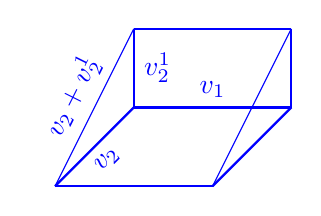
\begin{tikzpicture}
\draw[thick,blue] (2,2) to [edge node = {node [above] {$v_1$}}] (4,2);
\draw[thick,blue] (2,3) -- (4,3);
\draw[thick,blue] (2,2) to [edge node = {node [right] {$v_2^1$}}] (2,3);
\draw[thick,blue] (4,2) -- (4,3);
\draw[thick,blue] (1,1) to [edge node = {node [sloped,below] {$v_2$}}] (2,2);
\draw[thick,blue] (3,1) -- (4,2);
\draw[thick,blue] (1,1) -- (3,1);
\draw[thin,blue] (1,1) to [edge node = {node [sloped,above] {$v_2+v_2^1$}}] (2,3);
\draw[thin,blue] (3,1) -- (4,3);
\end{tikzpicture}

One may view a matrix $A \in \Mat_n \left(\F\right)$ as an $n$-tuple of elements of $\F^n$ (its columns):
\begin{equation*}
\begin{aligned}
A = \left(A^{(1)},...,A^{(n)}\right)
\end{aligned}
\end{equation*}

\begin{lemma}
$\det$ is a volume form.
\begin{proof}
To see $\det$ is multi-linear, it suffices to see that 
\begin{equation*}
\begin{aligned}
\cap_{i=1}^n A_{i \sigma\left(1\right)}
\end{aligned}
\end{equation*}
is multilinear for each $\sigma \in S_n$, since any linear combination of (multi)-linear functions is also (multi)-linear.

But $\cap_{i=1}^n A_{i \sigma\left(1\right)}$ contains one entry from each column, so is clearly multi-linear.

Suppose $A^{(k)} = A^{(l)}$ for some $k \neq l$. Let $\tau = \left(kl\right)$. Then $A_{ij} = A_{i\tau\left(j\right)}$ for all $1 \leq i,j \leq n$.

But $S_n$ is the disjoint union of $A_n$ and $\tau A_n$, and
\begin{equation*}
\begin{aligned}
\sum_{\sigma \in A_n} \cap_{i=1}^n A_{i \sigma\left(i\right)} = \sum_{\sigma \in \tau A_n} \cap_{i=1}^n A_{i \sigma\left(i\right)}
\end{aligned}
\end{equation*}
so
\begin{equation*}
\begin{aligned}
\det A = LHS - RHS = 0
\end{aligned}
\end{equation*}
\end{proof}
\end{lemma}

\end{document}